\documentclass[twoside]{book}

% Packages required by doxygen
\usepackage{fixltx2e}
\usepackage{calc}
\usepackage{doxygen}
\usepackage[export]{adjustbox} % also loads graphicx
\usepackage{graphicx}
\usepackage[utf8]{inputenc}
\usepackage{makeidx}
\usepackage{multicol}
\usepackage{multirow}
\PassOptionsToPackage{warn}{textcomp}
\usepackage{textcomp}
\usepackage[nointegrals]{wasysym}
\usepackage[table]{xcolor}

% NLS support packages
\usepackage[T2A]{fontenc}
\usepackage[czech]{babel}

% Font selection
\usepackage[T1]{fontenc}
\usepackage[scaled=.90]{helvet}
\usepackage{courier}
\usepackage{amssymb}
\usepackage{sectsty}
\renewcommand{\familydefault}{\sfdefault}
\allsectionsfont{%
  \fontseries{bc}\selectfont%
  \color{darkgray}%
}
\renewcommand{\DoxyLabelFont}{%
  \fontseries{bc}\selectfont%
  \color{darkgray}%
}
\newcommand{\+}{\discretionary{\mbox{\scriptsize$\hookleftarrow$}}{}{}}

% Page & text layout
\usepackage{geometry}
\geometry{%
  a4paper,%
  top=2.5cm,%
  bottom=2.5cm,%
  left=2.5cm,%
  right=2.5cm%
}
\tolerance=750
\hfuzz=15pt
\hbadness=750
\setlength{\emergencystretch}{15pt}
\setlength{\parindent}{0cm}
\setlength{\parskip}{3ex plus 2ex minus 2ex}
\makeatletter
\renewcommand{\paragraph}{%
  \@startsection{paragraph}{4}{0ex}{-1.0ex}{1.0ex}{%
    \normalfont\normalsize\bfseries\SS@parafont%
  }%
}
\renewcommand{\subparagraph}{%
  \@startsection{subparagraph}{5}{0ex}{-1.0ex}{1.0ex}{%
    \normalfont\normalsize\bfseries\SS@subparafont%
  }%
}
\makeatother

% Headers & footers
\usepackage{fancyhdr}
\pagestyle{fancyplain}
\fancyhead[LE]{\fancyplain{}{\bfseries\thepage}}
\fancyhead[CE]{\fancyplain{}{}}
\fancyhead[RE]{\fancyplain{}{\bfseries\leftmark}}
\fancyhead[LO]{\fancyplain{}{\bfseries\rightmark}}
\fancyhead[CO]{\fancyplain{}{}}
\fancyhead[RO]{\fancyplain{}{\bfseries\thepage}}
\fancyfoot[LE]{\fancyplain{}{}}
\fancyfoot[CE]{\fancyplain{}{}}
\fancyfoot[RE]{\fancyplain{}{\bfseries\scriptsize Generováno programem Doxygen }}
\fancyfoot[LO]{\fancyplain{}{\bfseries\scriptsize Generováno programem Doxygen }}
\fancyfoot[CO]{\fancyplain{}{}}
\fancyfoot[RO]{\fancyplain{}{}}
\renewcommand{\footrulewidth}{0.4pt}
\renewcommand{\chaptermark}[1]{%
  \markboth{#1}{}%
}
\renewcommand{\sectionmark}[1]{%
  \markright{\thesection\ #1}%
}

% Indices & bibliography
\usepackage{natbib}
\usepackage[titles]{tocloft}
\setcounter{tocdepth}{3}
\setcounter{secnumdepth}{5}
\makeindex

% Hyperlinks (required, but should be loaded last)
\usepackage{ifpdf}
\ifpdf
  \usepackage[pdftex,pagebackref=true]{hyperref}
\else
  \usepackage[ps2pdf,pagebackref=true]{hyperref}
\fi
\hypersetup{%
  colorlinks=true,%
  linkcolor=blue,%
  citecolor=blue,%
  unicode%
}

% Custom commands
\newcommand{\clearemptydoublepage}{%
  \newpage{\pagestyle{empty}\cleardoublepage}%
}

\usepackage{caption}
\captionsetup{labelsep=space,justification=centering,font={bf},singlelinecheck=off,skip=4pt,position=top}

%===== C O N T E N T S =====

\begin{document}

% Titlepage & ToC
\hypersetup{pageanchor=false,
             bookmarksnumbered=true,
             pdfencoding=unicode
            }
\pagenumbering{roman}
\begin{titlepage}
\vspace*{7cm}
\begin{center}%
{\Large Seki \\[1ex]\large v.\+1.\+2 }\\
\vspace*{1cm}
{\large Generováno programem Doxygen 1.8.11}\\
\end{center}
\end{titlepage}
\clearemptydoublepage
\tableofcontents
\clearemptydoublepage
\pagenumbering{arabic}
\hypersetup{pageanchor=true}

%--- Begin generated contents ---
\chapter{Rejstřík tříd}
\section{Seznam tříd}
Následující seznam obsahuje především identifikace tříd, ale nacházejí se zde i další netriviální prvky, jako jsou struktury (struct), unie (union) a rozhraní (interface). V seznamu jsou uvedeny jejich stručné popisy\+:\begin{DoxyCompactList}
\item\contentsline{section}{\hyperlink{class_bluetooth}{Bluetooth} }{\pageref{class_bluetooth}}{}
\item\contentsline{section}{\hyperlink{class_ibt}{Ibt} }{\pageref{class_ibt}}{}
\item\contentsline{section}{\hyperlink{class_sekacka}{Sekacka} }{\pageref{class_sekacka}}{}
\end{DoxyCompactList}

\chapter{Rejstřík souborů}
\section{Seznam souborů}
Zde naleznete seznam všech dokumentovaných souborů se stručnými popisy\+:\begin{DoxyCompactList}
\item\contentsline{section}{\hyperlink{bluetooth_8h}{bluetooth.\+h} }{\pageref{bluetooth_8h}}{}
\item\contentsline{section}{\hyperlink{drivers_8h}{drivers.\+h} }{\pageref{drivers_8h}}{}
\item\contentsline{section}{\hyperlink{ibt_8h}{ibt.\+h} }{\pageref{ibt_8h}}{}
\item\contentsline{section}{\hyperlink{sekacka_8h}{sekacka.\+h} }{\pageref{sekacka_8h}}{}
\end{DoxyCompactList}

\chapter{Dokumentace tříd}
\hypertarget{class_bluetooth}{}\section{Dokumentace třídy Bluetooth}
\label{class_bluetooth}\index{Bluetooth@{Bluetooth}}
\subsection*{Veřejné metody}
\begin{DoxyCompactItemize}
\item 
\hyperlink{class_bluetooth_adff22f9e5f2bd81b1fc5b8eeba71f68b}{Bluetooth} ()
\item 
void \hyperlink{class_bluetooth_a2d038a039804b49420b4361dadca5f03}{write\+BT} (String s)
\item 
char \hyperlink{class_bluetooth_acf117626c09166fa644283fab63b91e0}{read\+BT} ()
\item 
void \hyperlink{class_bluetooth_aac43de4109654ffd008a4ad10a7073b1}{set\+Name} (String name)
\item 
void \hyperlink{class_bluetooth_aca52b5e2fd06c4868a8f17ef5c3d6e20}{set\+Pin} (int pin)
\item 
bool \hyperlink{class_bluetooth_a32206b7170e65b05b30999d8c628f81e}{is\+Con} ()
\end{DoxyCompactItemize}
\subsection*{Privátní atributy}
\begin{DoxyCompactItemize}
\item 
char \hyperlink{class_bluetooth_adef51eff78a48180af18bb59bbfe9702}{bt\+Data}
\item 
long \hyperlink{class_bluetooth_a4c50a5cea29bb234f37aba4c8632d0b2}{bt\+Rate}
\end{DoxyCompactItemize}


\subsection{Dokumentace konstruktoru a destruktoru}
\index{Bluetooth@{Bluetooth}!Bluetooth@{Bluetooth}}
\index{Bluetooth@{Bluetooth}!Bluetooth@{Bluetooth}}
\subsubsection[{\texorpdfstring{Bluetooth()}{Bluetooth()}}]{\setlength{\rightskip}{0pt plus 5cm}Bluetooth\+::\+Bluetooth (
\begin{DoxyParamCaption}
{}
\end{DoxyParamCaption}
)}\hypertarget{class_bluetooth_adff22f9e5f2bd81b1fc5b8eeba71f68b}{}\label{class_bluetooth_adff22f9e5f2bd81b1fc5b8eeba71f68b}
A constructor 

\subsection{Dokumentace k metodám}
\index{Bluetooth@{Bluetooth}!is\+Con@{is\+Con}}
\index{is\+Con@{is\+Con}!Bluetooth@{Bluetooth}}
\subsubsection[{\texorpdfstring{is\+Con()}{isCon()}}]{\setlength{\rightskip}{0pt plus 5cm}bool Bluetooth\+::is\+Con (
\begin{DoxyParamCaption}
{}
\end{DoxyParamCaption}
)}\hypertarget{class_bluetooth_a32206b7170e65b05b30999d8c628f81e}{}\label{class_bluetooth_a32206b7170e65b05b30999d8c628f81e}
Metoda vrací zda je serial avaible \begin{DoxyReturn}{Návratová hodnota}
bool je serial aveible 
\end{DoxyReturn}
\index{Bluetooth@{Bluetooth}!read\+BT@{read\+BT}}
\index{read\+BT@{read\+BT}!Bluetooth@{Bluetooth}}
\subsubsection[{\texorpdfstring{read\+B\+T()}{readBT()}}]{\setlength{\rightskip}{0pt plus 5cm}char Bluetooth\+::read\+BT (
\begin{DoxyParamCaption}
{}
\end{DoxyParamCaption}
)}\hypertarget{class_bluetooth_acf117626c09166fa644283fab63b91e0}{}\label{class_bluetooth_acf117626c09166fa644283fab63b91e0}
Metoda čte seriovou linku \index{Bluetooth@{Bluetooth}!set\+Name@{set\+Name}}
\index{set\+Name@{set\+Name}!Bluetooth@{Bluetooth}}
\subsubsection[{\texorpdfstring{set\+Name(\+String name)}{setName(String name)}}]{\setlength{\rightskip}{0pt plus 5cm}void Bluetooth\+::set\+Name (
\begin{DoxyParamCaption}
\item[{String}]{name}
\end{DoxyParamCaption}
)}\hypertarget{class_bluetooth_aac43de4109654ffd008a4ad10a7073b1}{}\label{class_bluetooth_aac43de4109654ffd008a4ad10a7073b1}
Metoda nastaví jméno modulu H\+C-\/06 
\begin{DoxyParams}{Parametry}
{\em name} & type String nazev bluetooth modulu \\
\hline
\end{DoxyParams}
\index{Bluetooth@{Bluetooth}!set\+Pin@{set\+Pin}}
\index{set\+Pin@{set\+Pin}!Bluetooth@{Bluetooth}}
\subsubsection[{\texorpdfstring{set\+Pin(int pin)}{setPin(int pin)}}]{\setlength{\rightskip}{0pt plus 5cm}void Bluetooth\+::set\+Pin (
\begin{DoxyParamCaption}
\item[{int}]{pin}
\end{DoxyParamCaption}
)}\hypertarget{class_bluetooth_aca52b5e2fd06c4868a8f17ef5c3d6e20}{}\label{class_bluetooth_aca52b5e2fd06c4868a8f17ef5c3d6e20}
Metoda nastaví pin modulu H\+C-\/06 
\begin{DoxyParams}{Parametry}
{\em pin} & type int heslo pro bluetooth modul \\
\hline
\end{DoxyParams}
\index{Bluetooth@{Bluetooth}!write\+BT@{write\+BT}}
\index{write\+BT@{write\+BT}!Bluetooth@{Bluetooth}}
\subsubsection[{\texorpdfstring{write\+B\+T(\+String s)}{writeBT(String s)}}]{\setlength{\rightskip}{0pt plus 5cm}void Bluetooth\+::write\+BT (
\begin{DoxyParamCaption}
\item[{String}]{s}
\end{DoxyParamCaption}
)}\hypertarget{class_bluetooth_a2d038a039804b49420b4361dadca5f03}{}\label{class_bluetooth_a2d038a039804b49420b4361dadca5f03}
Metoda která zapisuje hodnotu v parametru na seriovou linku připojenou k bloutooth modulu 
\begin{DoxyParams}{Parametry}
{\em s} & type string string se vypíše na seriovou linku \\
\hline
\end{DoxyParams}


\subsection{Dokumentace k datovým členům}
\index{Bluetooth@{Bluetooth}!bt\+Data@{bt\+Data}}
\index{bt\+Data@{bt\+Data}!Bluetooth@{Bluetooth}}
\subsubsection[{\texorpdfstring{bt\+Data}{btData}}]{\setlength{\rightskip}{0pt plus 5cm}char Bluetooth\+::bt\+Data\hspace{0.3cm}{\ttfamily [private]}}\hypertarget{class_bluetooth_adef51eff78a48180af18bb59bbfe9702}{}\label{class_bluetooth_adef51eff78a48180af18bb59bbfe9702}
proměnná pro čtení z seriové liky \index{Bluetooth@{Bluetooth}!bt\+Rate@{bt\+Rate}}
\index{bt\+Rate@{bt\+Rate}!Bluetooth@{Bluetooth}}
\subsubsection[{\texorpdfstring{bt\+Rate}{btRate}}]{\setlength{\rightskip}{0pt plus 5cm}long Bluetooth\+::bt\+Rate\hspace{0.3cm}{\ttfamily [private]}}\hypertarget{class_bluetooth_a4c50a5cea29bb234f37aba4c8632d0b2}{}\label{class_bluetooth_a4c50a5cea29bb234f37aba4c8632d0b2}
hodnota bychlosti seriové liky pro modul bluetooth 

Dokumentace pro tuto třídu byla generována z následujících souborů\+:\begin{DoxyCompactItemize}
\item 
\hyperlink{bluetooth_8h}{bluetooth.\+h}\item 
bluetooth.\+cpp\end{DoxyCompactItemize}

\hypertarget{class_ibt}{}\section{Dokumentace třídy Ibt}
\label{class_ibt}\index{Ibt@{Ibt}}
\subsection*{Veřejné metody}
\begin{DoxyCompactItemize}
\item 
\hyperlink{class_ibt_a7095837f79f0d4329a6f44b54480c26e}{Ibt} (int \hyperlink{class_ibt_ad6d59ade8bcb80ee7ee06c475a381dea}{pin\+Motor\+Enable}, int \hyperlink{class_ibt_a7112beac87f2013be51d48203e23a1f5}{pin\+Motor\+P\+W\+MR}, int \hyperlink{class_ibt_a392b4ea56f7346c43b9562e77fe35722}{pin\+Motor\+P\+W\+ML}, int \hyperlink{class_ibt_ac52829806ce90d85f76320292e7027a4}{pin\+Motor\+Sense})
\item 
void \hyperlink{class_ibt_ad5096d0ae4d1d1ce3714868f2f4b3fec}{set\+Data} (bool \hyperlink{class_ibt_ab15472546c05e0760f6a1b282fad58fb}{smer}, int \hyperlink{class_ibt_a8e62674f6908473dc87800a656142d7c}{value})
\item 
void \hyperlink{class_ibt_ade1b0109381b41dc9cd254de475a6c16}{set\+Stop} ()
\item 
void \hyperlink{class_ibt_abf510206cd1ab3c5067fd1662a1e63f2}{aplikovat} ()
\item 
bool \hyperlink{class_ibt_ad1c2a7fa28e908578fa73f1978c3f0c5}{get\+Smer} ()
\item 
int \hyperlink{class_ibt_ab4b9fec5dcc3520653d1d42482a36f80}{get\+Value} ()
\end{DoxyCompactItemize}
\subsection*{Privátní atributy}
\begin{DoxyCompactItemize}
\item 
int \hyperlink{class_ibt_ad6d59ade8bcb80ee7ee06c475a381dea}{pin\+Motor\+Enable}
\item 
int \hyperlink{class_ibt_a392b4ea56f7346c43b9562e77fe35722}{pin\+Motor\+P\+W\+ML}
\item 
int \hyperlink{class_ibt_a7112beac87f2013be51d48203e23a1f5}{pin\+Motor\+P\+W\+MR}
\item 
int \hyperlink{class_ibt_ac52829806ce90d85f76320292e7027a4}{pin\+Motor\+Sense}
\item 
bool \hyperlink{class_ibt_ab15472546c05e0760f6a1b282fad58fb}{smer}
\item 
int \hyperlink{class_ibt_a8e62674f6908473dc87800a656142d7c}{value}
\end{DoxyCompactItemize}


\subsection{Dokumentace konstruktoru a destruktoru}
\index{Ibt@{Ibt}!Ibt@{Ibt}}
\index{Ibt@{Ibt}!Ibt@{Ibt}}
\subsubsection[{\texorpdfstring{Ibt(int pin\+Motor\+Enable, int pin\+Motor\+P\+W\+M\+R, int pin\+Motor\+P\+W\+M\+L, int pin\+Motor\+Sense)}{Ibt(int pinMotorEnable, int pinMotorPWMR, int pinMotorPWML, int pinMotorSense)}}]{\setlength{\rightskip}{0pt plus 5cm}Ibt\+::\+Ibt (
\begin{DoxyParamCaption}
\item[{int}]{pin\+Motor\+Enable, }
\item[{int}]{pin\+Motor\+P\+W\+MR, }
\item[{int}]{pin\+Motor\+P\+W\+ML, }
\item[{int}]{pin\+Motor\+Sense}
\end{DoxyParamCaption}
)}\hypertarget{class_ibt_a7095837f79f0d4329a6f44b54480c26e}{}\label{class_ibt_a7095837f79f0d4329a6f44b54480c26e}
A constructor. 
\begin{DoxyParams}{Parametry}
{\em pin\+Motor\+Left\+Enable} & pin na kterém je enable \\
\hline
{\em pin\+Motor\+P\+W\+ML} & pin na který budeme posílat P\+WM pro jízdu jedním směrem \\
\hline
{\em pin\+Motor\+P\+W\+MR} & pin na který budeme posílat P\+WM pro jízdu druhým směrem \\
\hline
{\em pin\+Motor\+Sense} & pin kterým probíhá čtení aktuálního proudu regulátoru \\
\hline
\end{DoxyParams}


\subsection{Dokumentace k metodám}
\index{Ibt@{Ibt}!aplikovat@{aplikovat}}
\index{aplikovat@{aplikovat}!Ibt@{Ibt}}
\subsubsection[{\texorpdfstring{aplikovat()}{aplikovat()}}]{\setlength{\rightskip}{0pt plus 5cm}void Ibt\+::aplikovat (
\begin{DoxyParamCaption}
{}
\end{DoxyParamCaption}
)}\hypertarget{class_ibt_abf510206cd1ab3c5067fd1662a1e63f2}{}\label{class_ibt_abf510206cd1ab3c5067fd1662a1e63f2}
Metoda která aplikuje privátní proměnné k danému výstupu. \index{Ibt@{Ibt}!get\+Smer@{get\+Smer}}
\index{get\+Smer@{get\+Smer}!Ibt@{Ibt}}
\subsubsection[{\texorpdfstring{get\+Smer()}{getSmer()}}]{\setlength{\rightskip}{0pt plus 5cm}bool Ibt\+::get\+Smer (
\begin{DoxyParamCaption}
{}
\end{DoxyParamCaption}
)}\hypertarget{class_ibt_ad1c2a7fa28e908578fa73f1978c3f0c5}{}\label{class_ibt_ad1c2a7fa28e908578fa73f1978c3f0c5}
Metoda vypisuje členská data S\+M\+ER \index{Ibt@{Ibt}!get\+Value@{get\+Value}}
\index{get\+Value@{get\+Value}!Ibt@{Ibt}}
\subsubsection[{\texorpdfstring{get\+Value()}{getValue()}}]{\setlength{\rightskip}{0pt plus 5cm}int Ibt\+::get\+Value (
\begin{DoxyParamCaption}
{}
\end{DoxyParamCaption}
)}\hypertarget{class_ibt_ab4b9fec5dcc3520653d1d42482a36f80}{}\label{class_ibt_ab4b9fec5dcc3520653d1d42482a36f80}
Metoda vypisuje členská data V\+A\+L\+UE \index{Ibt@{Ibt}!set\+Data@{set\+Data}}
\index{set\+Data@{set\+Data}!Ibt@{Ibt}}
\subsubsection[{\texorpdfstring{set\+Data(bool smer, int value)}{setData(bool smer, int value)}}]{\setlength{\rightskip}{0pt plus 5cm}void Ibt\+::set\+Data (
\begin{DoxyParamCaption}
\item[{bool}]{smer, }
\item[{int}]{value}
\end{DoxyParamCaption}
)}\hypertarget{class_ibt_ad5096d0ae4d1d1ce3714868f2f4b3fec}{}\label{class_ibt_ad5096d0ae4d1d1ce3714868f2f4b3fec}
Metoda která nadstavuje privátní proměnné třídy 
\begin{DoxyParams}{Parametry}
{\em směr} & type bool -\/ 1 vpřed -\/ 0 vzad \\
\hline
{\em value} & type int hodnota výstupního proudu z regulátoru v P\+WM od 0 do 255 \\
\hline
\end{DoxyParams}
\index{Ibt@{Ibt}!set\+Stop@{set\+Stop}}
\index{set\+Stop@{set\+Stop}!Ibt@{Ibt}}
\subsubsection[{\texorpdfstring{set\+Stop()}{setStop()}}]{\setlength{\rightskip}{0pt plus 5cm}void Ibt\+::set\+Stop (
\begin{DoxyParamCaption}
{}
\end{DoxyParamCaption}
)}\hypertarget{class_ibt_ade1b0109381b41dc9cd254de475a6c16}{}\label{class_ibt_ade1b0109381b41dc9cd254de475a6c16}
Metoda která nastaví privátní proměnné pro pohyb na 0 a směr 0 

\subsection{Dokumentace k datovým členům}
\index{Ibt@{Ibt}!pin\+Motor\+Enable@{pin\+Motor\+Enable}}
\index{pin\+Motor\+Enable@{pin\+Motor\+Enable}!Ibt@{Ibt}}
\subsubsection[{\texorpdfstring{pin\+Motor\+Enable}{pinMotorEnable}}]{\setlength{\rightskip}{0pt plus 5cm}int Ibt\+::pin\+Motor\+Enable\hspace{0.3cm}{\ttfamily [private]}}\hypertarget{class_ibt_ad6d59ade8bcb80ee7ee06c475a381dea}{}\label{class_ibt_ad6d59ade8bcb80ee7ee06c475a381dea}
na kterém pinu se nachází enable \index{Ibt@{Ibt}!pin\+Motor\+P\+W\+ML@{pin\+Motor\+P\+W\+ML}}
\index{pin\+Motor\+P\+W\+ML@{pin\+Motor\+P\+W\+ML}!Ibt@{Ibt}}
\subsubsection[{\texorpdfstring{pin\+Motor\+P\+W\+ML}{pinMotorPWML}}]{\setlength{\rightskip}{0pt plus 5cm}int Ibt\+::pin\+Motor\+P\+W\+ML\hspace{0.3cm}{\ttfamily [private]}}\hypertarget{class_ibt_a392b4ea56f7346c43b9562e77fe35722}{}\label{class_ibt_a392b4ea56f7346c43b9562e77fe35722}
pin na který se aplikuje pwm pro jízdu jedním směrem \index{Ibt@{Ibt}!pin\+Motor\+P\+W\+MR@{pin\+Motor\+P\+W\+MR}}
\index{pin\+Motor\+P\+W\+MR@{pin\+Motor\+P\+W\+MR}!Ibt@{Ibt}}
\subsubsection[{\texorpdfstring{pin\+Motor\+P\+W\+MR}{pinMotorPWMR}}]{\setlength{\rightskip}{0pt plus 5cm}int Ibt\+::pin\+Motor\+P\+W\+MR\hspace{0.3cm}{\ttfamily [private]}}\hypertarget{class_ibt_a7112beac87f2013be51d48203e23a1f5}{}\label{class_ibt_a7112beac87f2013be51d48203e23a1f5}
pin na který se aplikuje pwm pro jízdu druhým směrem \index{Ibt@{Ibt}!pin\+Motor\+Sense@{pin\+Motor\+Sense}}
\index{pin\+Motor\+Sense@{pin\+Motor\+Sense}!Ibt@{Ibt}}
\subsubsection[{\texorpdfstring{pin\+Motor\+Sense}{pinMotorSense}}]{\setlength{\rightskip}{0pt plus 5cm}int Ibt\+::pin\+Motor\+Sense\hspace{0.3cm}{\ttfamily [private]}}\hypertarget{class_ibt_ac52829806ce90d85f76320292e7027a4}{}\label{class_ibt_ac52829806ce90d85f76320292e7027a4}
pin na kterém měříme hodnotu napětí na regulátoru \index{Ibt@{Ibt}!smer@{smer}}
\index{smer@{smer}!Ibt@{Ibt}}
\subsubsection[{\texorpdfstring{smer}{smer}}]{\setlength{\rightskip}{0pt plus 5cm}bool Ibt\+::smer\hspace{0.3cm}{\ttfamily [private]}}\hypertarget{class_ibt_ab15472546c05e0760f6a1b282fad58fb}{}\label{class_ibt_ab15472546c05e0760f6a1b282fad58fb}
směr jízdy 1,0 \index{Ibt@{Ibt}!value@{value}}
\index{value@{value}!Ibt@{Ibt}}
\subsubsection[{\texorpdfstring{value}{value}}]{\setlength{\rightskip}{0pt plus 5cm}int Ibt\+::value\hspace{0.3cm}{\ttfamily [private]}}\hypertarget{class_ibt_a8e62674f6908473dc87800a656142d7c}{}\label{class_ibt_a8e62674f6908473dc87800a656142d7c}
hodnota P\+WM od 0 do 255 

Dokumentace pro tuto třídu byla generována z následujících souborů\+:\begin{DoxyCompactItemize}
\item 
\hyperlink{ibt_8h}{ibt.\+h}\item 
ibt.\+cpp\end{DoxyCompactItemize}

\hypertarget{class_sekacka}{}\section{Dokumentace třídy Sekacka}
\label{class_sekacka}\index{Sekacka@{Sekacka}}
\subsection*{Veřejné metody}
\begin{DoxyCompactItemize}
\item 
\hyperlink{class_sekacka_ab5821740b364c9fc32887f0fbef5d3ae}{Sekacka} ()
\item 
virtual void \hyperlink{class_sekacka_a2e38c70d8fdd55e112e42b4aa4afc14f}{setup} (void)
\item 
virtual void \hyperlink{class_sekacka_afd84d6e1644824b8cf317ea0514e8176}{loop} (void)
\end{DoxyCompactItemize}
\subsection*{Privátní typy}
\begin{DoxyCompactItemize}
\item 
enum \{ \\*
\hyperlink{class_sekacka_a4b9f99f468351377c74f1906012dddcead823d74f46614cb9d4c6256a47d52427}{F\+R\+O\+NT}, 
\hyperlink{class_sekacka_a4b9f99f468351377c74f1906012dddcea48ecf5835232244136c4f81df5843716}{F\+R\+O\+N\+T\+\_\+\+S\+L\+OW}, 
\hyperlink{class_sekacka_a4b9f99f468351377c74f1906012dddcea84850430a560bac207f0c6c43e5f6db3}{L\+E\+FT}, 
\hyperlink{class_sekacka_a4b9f99f468351377c74f1906012dddcea1e7fc60b9bccf54cce66fb95ce4381af}{B\+A\+CK}, 
\\*
\hyperlink{class_sekacka_a4b9f99f468351377c74f1906012dddcea78fa66f2894ab0692bd2da0aafd67ffd}{S\+T\+OP}
 \}
\item 
enum \{ \hyperlink{class_sekacka_aedeaa9da2c7ac3e0e3c4428aa4900e51a379a7e5f78b78b7648cae76ae7fbc68b}{S\+E\+N\+\_\+\+S\+O\+N\+A\+R\+\_\+\+C\+E\+N\+T\+E\+R\+\_\+\+L\+E\+FT}, 
\hyperlink{class_sekacka_aedeaa9da2c7ac3e0e3c4428aa4900e51adcf2288828acde8c4d12bf4822649b1d}{S\+E\+N\+\_\+\+S\+O\+N\+A\+R\+\_\+\+C\+E\+N\+T\+E\+R\+\_\+\+R\+I\+G\+HT}, 
\hyperlink{class_sekacka_aedeaa9da2c7ac3e0e3c4428aa4900e51afdaf5f1fef5da7d907721e6ecf8fa8cd}{S\+E\+N\+\_\+\+S\+O\+N\+A\+R\+\_\+\+L\+E\+FT}, 
\hyperlink{class_sekacka_aedeaa9da2c7ac3e0e3c4428aa4900e51aa4b8410a39bc42c19d5a57e269e3dc10}{S\+E\+N\+\_\+\+S\+O\+N\+A\+R\+\_\+\+R\+I\+G\+HT}
 \}
\item 
enum \{ \\*
\hyperlink{class_sekacka_a0edd5506d9ddcf2b4b243c985ecd5160a0cd5677d8ceffda417bcc18a781017b9}{M\+O\+T\+O\+R\+\_\+\+F\+R\+O\+NT}, 
\hyperlink{class_sekacka_a0edd5506d9ddcf2b4b243c985ecd5160a55b8b97cf76f21d488480a8eb873d200}{M\+O\+T\+O\+R\+\_\+\+F\+R\+O\+N\+T\+\_\+\+L\+E\+FT}, 
\hyperlink{class_sekacka_a0edd5506d9ddcf2b4b243c985ecd5160ac7548fd36c3ebc4fc29d3d7023880fab}{M\+O\+T\+O\+R\+\_\+\+F\+R\+O\+N\+T\+\_\+\+R\+I\+G\+HT}, 
\hyperlink{class_sekacka_a0edd5506d9ddcf2b4b243c985ecd5160a9e179057564e6515f78816d495ff0d0f}{M\+O\+T\+O\+R\+\_\+\+B\+A\+CK}, 
\\*
\hyperlink{class_sekacka_a0edd5506d9ddcf2b4b243c985ecd5160a0902d9742484c9c9e0a6eb5da8229eba}{M\+O\+T\+O\+R\+\_\+\+B\+A\+C\+K\+\_\+\+L\+E\+FT}, 
\hyperlink{class_sekacka_a0edd5506d9ddcf2b4b243c985ecd5160a110449350235a35afc101260af71b906}{M\+O\+T\+O\+R\+\_\+\+B\+A\+C\+K\+\_\+\+R\+I\+G\+HT}, 
\hyperlink{class_sekacka_a0edd5506d9ddcf2b4b243c985ecd5160a5b08a4031a954a7753fd8d81481fcd6c}{M\+O\+T\+O\+R\+\_\+\+L\+E\+FT}, 
\hyperlink{class_sekacka_a0edd5506d9ddcf2b4b243c985ecd5160a19115f90a2b8cb651933bc44ce9f1af2}{M\+O\+T\+O\+R\+\_\+\+R\+I\+G\+HT}, 
\\*
\hyperlink{class_sekacka_a0edd5506d9ddcf2b4b243c985ecd5160a507ecdc492d55c96b8e4bae21d49a360}{M\+O\+T\+O\+R\+\_\+\+S\+T\+OP}
 \}
\end{DoxyCompactItemize}
\subsection*{Privátní metody}
\begin{DoxyCompactItemize}
\item 
void \hyperlink{class_sekacka_a6a2fcbb0bf1c52c918abeae2e8f2f37b}{print\+Info} ()
\item 
void \hyperlink{class_sekacka_a1c1a72cdf2e70b8bbc8867d827a33c36}{read\+Sensors} ()
\item 
int \hyperlink{class_sekacka_a0f1c6b2e3749c0d20e8d030c4ca2f41e}{read\+Sensor} (char)
\item 
void \hyperlink{class_sekacka_ad8b987c58efd929f4a1ab6fb83228c12}{motor\+Pohyb} (char)
\item 
void \hyperlink{class_sekacka_a6bc30aad27b57ebcf8dfbc8c13064d71}{motor\+Update} ()
\item 
bool \hyperlink{class_sekacka_a93bcb289ba8a8a6edf49c44118c63948}{sonar\+Muzu} (char)
\item 
void \hyperlink{class_sekacka_a3b8a0b514630002f3f1cb4e2a82825d8}{print\+Menu} ()
\item 
void \hyperlink{class_sekacka_a4314290befcd561c07bc33a9fb8c2d23}{menu} ()
\item 
void \hyperlink{class_sekacka_adf78055c6bcd3211df182efb9571e596}{read\+Serial} ()
\item 
void \hyperlink{class_sekacka_ace29e111ad870829ec7a5581318d989d}{test\+Motors} ()
\item 
void \hyperlink{class_sekacka_a2f4b2d82d958ad109742d3d341f8b5a4}{test\+Sonar} ()
\item 
void \hyperlink{class_sekacka_a31d02cd2da2b004f24cd5a7c18290824}{read\+Bluetooth} ()
\end{DoxyCompactItemize}
\subsection*{Privátní atributy}
\begin{DoxyCompactItemize}
\item 
int \hyperlink{class_sekacka_a41aa8e032754f0b39f3d86583972e9ca}{use\+Print\+Info}
\item 
unsigned long \hyperlink{class_sekacka_a34c88c43f0c6573f8005d7d40ccbec75}{start\+Time}
\item 
unsigned long \hyperlink{class_sekacka_ad1a2be8445580ee6da05f49c0d7905e9}{next\+Time\+Info}
\item 
int \hyperlink{class_sekacka_a796c17e80ad5c084b336197e609c2f0e}{update\+Time\+Info}
\item 
unsigned long \hyperlink{class_sekacka_a3d40897d033fe36d1644520562a3c497}{next\+Time\+Motor}
\item 
int \hyperlink{class_sekacka_a8d00207d9eeb49ca50dcf1cfae2bf89a}{update\+Time\+Motor}
\item 
int \hyperlink{class_sekacka_a0407757c0371f299eac49abf5feb1f77}{time\+Update\+Time}
\item 
int \hyperlink{class_sekacka_a82a00364ae6395253285518471f3132b}{time\+Rotage}
\item 
int \hyperlink{class_sekacka_a87ae7490a2de5bfd9f8a6e5e2f09b207}{time\+Rotage\+Motor}
\item 
bool \hyperlink{class_sekacka_aa135507dbc52a6c2dd6e9f6ff2457b36}{drive}
\item 
char \hyperlink{class_sekacka_a518f65b47b3cd448734ee0a0022cfea1}{char\+Bluetooth}
\item 
char \hyperlink{class_sekacka_a64d54c86f397f9c2bf469dabb8d82176}{sonar\+Use}
\item 
char \hyperlink{class_sekacka_a78af23ffa04ade64990fa72c8ae10543}{sonar\+Left\+Use}
\item 
char \hyperlink{class_sekacka_a742636442a58009b65d5ddfce21333b8}{sonar\+Right\+Use}
\item 
char \hyperlink{class_sekacka_aa1dda76e93ca7282a9ae50dc4f980301}{sonar\+Center\+Right\+Use}
\item 
char \hyperlink{class_sekacka_aa43c6437efd1edbcfdbb22496ed4a226}{sonar\+Center\+Left\+Use}
\item 
unsigned int \hyperlink{class_sekacka_ac854e19a9eb8d30384f5ab0cdcdbaebf}{sonar\+Dist\+Center\+Left}
\item 
unsigned int \hyperlink{class_sekacka_ac9d9f43f254129e928f8855847132de0}{sonar\+Dist\+Center\+Right}
\item 
unsigned int \hyperlink{class_sekacka_a207ffc8368c5d5fe4d43efeed0c924d0}{sonar\+Dist\+Right}
\item 
unsigned int \hyperlink{class_sekacka_ab7bdf6c96058d419c7d98b02893df638}{sonar\+Dist\+Left}
\item 
unsigned long \hyperlink{class_sekacka_a0ef81f7686a22c5f4e7fa004dfa14930}{next\+Time\+Sonar}
\item 
int \hyperlink{class_sekacka_ad2f7b8a0daa12b6749f0e6d3fc72987a}{dist\+Min}
\item 
int \hyperlink{class_sekacka_a129f7eb9e4d1476fcc40ed610604132a}{dist\+Slow}
\end{DoxyCompactItemize}


\subsection{Dokumentace k členským výčtům}
\subsubsection[{\texorpdfstring{anonymous enum}{anonymous enum}}]{\setlength{\rightskip}{0pt plus 5cm}anonymous enum\hspace{0.3cm}{\ttfamily [private]}}\hypertarget{class_sekacka_a4b9f99f468351377c74f1906012dddce}{}\label{class_sekacka_a4b9f99f468351377c74f1906012dddce}
Enum pro povolení jízdy od senzoru určení směru jízdy, použití pro senzory aby určili vzdálenost pro jístu v daném směru \begin{Desc}
\item[Hodnoty výčtu]\par
\begin{description}
\index{F\+R\+O\+NT@{F\+R\+O\+NT}!Sekacka@{Sekacka}}\index{Sekacka@{Sekacka}!F\+R\+O\+NT@{F\+R\+O\+NT}}\item[{\em 
F\+R\+O\+NT\hypertarget{class_sekacka_a4b9f99f468351377c74f1906012dddcead823d74f46614cb9d4c6256a47d52427}{}\label{class_sekacka_a4b9f99f468351377c74f1906012dddcead823d74f46614cb9d4c6256a47d52427}
}]enum value F\+R\+O\+NT. \index{F\+R\+O\+N\+T\+\_\+\+S\+L\+OW@{F\+R\+O\+N\+T\+\_\+\+S\+L\+OW}!Sekacka@{Sekacka}}\index{Sekacka@{Sekacka}!F\+R\+O\+N\+T\+\_\+\+S\+L\+OW@{F\+R\+O\+N\+T\+\_\+\+S\+L\+OW}}\item[{\em 
F\+R\+O\+N\+T\+\_\+\+S\+L\+OW\hypertarget{class_sekacka_a4b9f99f468351377c74f1906012dddcea48ecf5835232244136c4f81df5843716}{}\label{class_sekacka_a4b9f99f468351377c74f1906012dddcea48ecf5835232244136c4f81df5843716}
}]enum value F\+R\+O\+N\+T\+\_\+\+S\+L\+OW. \index{L\+E\+FT@{L\+E\+FT}!Sekacka@{Sekacka}}\index{Sekacka@{Sekacka}!L\+E\+FT@{L\+E\+FT}}\item[{\em 
L\+E\+FT\hypertarget{class_sekacka_a4b9f99f468351377c74f1906012dddcea84850430a560bac207f0c6c43e5f6db3}{}\label{class_sekacka_a4b9f99f468351377c74f1906012dddcea84850430a560bac207f0c6c43e5f6db3}
}]enum value L\+E\+FT. \index{B\+A\+CK@{B\+A\+CK}!Sekacka@{Sekacka}}\index{Sekacka@{Sekacka}!B\+A\+CK@{B\+A\+CK}}\item[{\em 
B\+A\+CK\hypertarget{class_sekacka_a4b9f99f468351377c74f1906012dddcea1e7fc60b9bccf54cce66fb95ce4381af}{}\label{class_sekacka_a4b9f99f468351377c74f1906012dddcea1e7fc60b9bccf54cce66fb95ce4381af}
}]enum value B\+A\+CK. \index{S\+T\+OP@{S\+T\+OP}!Sekacka@{Sekacka}}\index{Sekacka@{Sekacka}!S\+T\+OP@{S\+T\+OP}}\item[{\em 
S\+T\+OP\hypertarget{class_sekacka_a4b9f99f468351377c74f1906012dddcea78fa66f2894ab0692bd2da0aafd67ffd}{}\label{class_sekacka_a4b9f99f468351377c74f1906012dddcea78fa66f2894ab0692bd2da0aafd67ffd}
}]enum value S\+T\+OP. \end{description}
\end{Desc}
\subsubsection[{\texorpdfstring{anonymous enum}{anonymous enum}}]{\setlength{\rightskip}{0pt plus 5cm}anonymous enum\hspace{0.3cm}{\ttfamily [private]}}\hypertarget{class_sekacka_aedeaa9da2c7ac3e0e3c4428aa4900e51}{}\label{class_sekacka_aedeaa9da2c7ac3e0e3c4428aa4900e51}
Enum pro určení senzoru slouží k rozpoznání seznosru od sebe \begin{Desc}
\item[Hodnoty výčtu]\par
\begin{description}
\index{S\+E\+N\+\_\+\+S\+O\+N\+A\+R\+\_\+\+C\+E\+N\+T\+E\+R\+\_\+\+L\+E\+FT@{S\+E\+N\+\_\+\+S\+O\+N\+A\+R\+\_\+\+C\+E\+N\+T\+E\+R\+\_\+\+L\+E\+FT}!Sekacka@{Sekacka}}\index{Sekacka@{Sekacka}!S\+E\+N\+\_\+\+S\+O\+N\+A\+R\+\_\+\+C\+E\+N\+T\+E\+R\+\_\+\+L\+E\+FT@{S\+E\+N\+\_\+\+S\+O\+N\+A\+R\+\_\+\+C\+E\+N\+T\+E\+R\+\_\+\+L\+E\+FT}}\item[{\em 
S\+E\+N\+\_\+\+S\+O\+N\+A\+R\+\_\+\+C\+E\+N\+T\+E\+R\+\_\+\+L\+E\+FT\hypertarget{class_sekacka_aedeaa9da2c7ac3e0e3c4428aa4900e51a379a7e5f78b78b7648cae76ae7fbc68b}{}\label{class_sekacka_aedeaa9da2c7ac3e0e3c4428aa4900e51a379a7e5f78b78b7648cae76ae7fbc68b}
}]enum value S\+E\+N\+\_\+\+S\+O\+N\+A\+R\+\_\+\+C\+E\+N\+T\+E\+R\+\_\+\+L\+E\+FT. \index{S\+E\+N\+\_\+\+S\+O\+N\+A\+R\+\_\+\+C\+E\+N\+T\+E\+R\+\_\+\+R\+I\+G\+HT@{S\+E\+N\+\_\+\+S\+O\+N\+A\+R\+\_\+\+C\+E\+N\+T\+E\+R\+\_\+\+R\+I\+G\+HT}!Sekacka@{Sekacka}}\index{Sekacka@{Sekacka}!S\+E\+N\+\_\+\+S\+O\+N\+A\+R\+\_\+\+C\+E\+N\+T\+E\+R\+\_\+\+R\+I\+G\+HT@{S\+E\+N\+\_\+\+S\+O\+N\+A\+R\+\_\+\+C\+E\+N\+T\+E\+R\+\_\+\+R\+I\+G\+HT}}\item[{\em 
S\+E\+N\+\_\+\+S\+O\+N\+A\+R\+\_\+\+C\+E\+N\+T\+E\+R\+\_\+\+R\+I\+G\+HT\hypertarget{class_sekacka_aedeaa9da2c7ac3e0e3c4428aa4900e51adcf2288828acde8c4d12bf4822649b1d}{}\label{class_sekacka_aedeaa9da2c7ac3e0e3c4428aa4900e51adcf2288828acde8c4d12bf4822649b1d}
}]enum value S\+E\+N\+\_\+\+S\+O\+N\+A\+R\+\_\+\+C\+E\+N\+T\+E\+R\+\_\+\+R\+I\+G\+HT. \index{S\+E\+N\+\_\+\+S\+O\+N\+A\+R\+\_\+\+L\+E\+FT@{S\+E\+N\+\_\+\+S\+O\+N\+A\+R\+\_\+\+L\+E\+FT}!Sekacka@{Sekacka}}\index{Sekacka@{Sekacka}!S\+E\+N\+\_\+\+S\+O\+N\+A\+R\+\_\+\+L\+E\+FT@{S\+E\+N\+\_\+\+S\+O\+N\+A\+R\+\_\+\+L\+E\+FT}}\item[{\em 
S\+E\+N\+\_\+\+S\+O\+N\+A\+R\+\_\+\+L\+E\+FT\hypertarget{class_sekacka_aedeaa9da2c7ac3e0e3c4428aa4900e51afdaf5f1fef5da7d907721e6ecf8fa8cd}{}\label{class_sekacka_aedeaa9da2c7ac3e0e3c4428aa4900e51afdaf5f1fef5da7d907721e6ecf8fa8cd}
}]enum value S\+E\+N\+\_\+\+S\+O\+N\+A\+R\+\_\+\+L\+E\+FT. \index{S\+E\+N\+\_\+\+S\+O\+N\+A\+R\+\_\+\+R\+I\+G\+HT@{S\+E\+N\+\_\+\+S\+O\+N\+A\+R\+\_\+\+R\+I\+G\+HT}!Sekacka@{Sekacka}}\index{Sekacka@{Sekacka}!S\+E\+N\+\_\+\+S\+O\+N\+A\+R\+\_\+\+R\+I\+G\+HT@{S\+E\+N\+\_\+\+S\+O\+N\+A\+R\+\_\+\+R\+I\+G\+HT}}\item[{\em 
S\+E\+N\+\_\+\+S\+O\+N\+A\+R\+\_\+\+R\+I\+G\+HT\hypertarget{class_sekacka_aedeaa9da2c7ac3e0e3c4428aa4900e51aa4b8410a39bc42c19d5a57e269e3dc10}{}\label{class_sekacka_aedeaa9da2c7ac3e0e3c4428aa4900e51aa4b8410a39bc42c19d5a57e269e3dc10}
}]enum value S\+E\+N\+\_\+\+S\+O\+N\+A\+R\+\_\+\+R\+I\+G\+HT. \end{description}
\end{Desc}
\subsubsection[{\texorpdfstring{anonymous enum}{anonymous enum}}]{\setlength{\rightskip}{0pt plus 5cm}anonymous enum\hspace{0.3cm}{\ttfamily [private]}}\hypertarget{class_sekacka_a0edd5506d9ddcf2b4b243c985ecd5160}{}\label{class_sekacka_a0edd5506d9ddcf2b4b243c985ecd5160}
Enum pro urční směru jízdy určuje směr jízdy \begin{Desc}
\item[Hodnoty výčtu]\par
\begin{description}
\index{M\+O\+T\+O\+R\+\_\+\+F\+R\+O\+NT@{M\+O\+T\+O\+R\+\_\+\+F\+R\+O\+NT}!Sekacka@{Sekacka}}\index{Sekacka@{Sekacka}!M\+O\+T\+O\+R\+\_\+\+F\+R\+O\+NT@{M\+O\+T\+O\+R\+\_\+\+F\+R\+O\+NT}}\item[{\em 
M\+O\+T\+O\+R\+\_\+\+F\+R\+O\+NT\hypertarget{class_sekacka_a0edd5506d9ddcf2b4b243c985ecd5160a0cd5677d8ceffda417bcc18a781017b9}{}\label{class_sekacka_a0edd5506d9ddcf2b4b243c985ecd5160a0cd5677d8ceffda417bcc18a781017b9}
}]enum value M\+O\+T\+O\+R\+\_\+\+F\+R\+O\+NT. \index{M\+O\+T\+O\+R\+\_\+\+F\+R\+O\+N\+T\+\_\+\+L\+E\+FT@{M\+O\+T\+O\+R\+\_\+\+F\+R\+O\+N\+T\+\_\+\+L\+E\+FT}!Sekacka@{Sekacka}}\index{Sekacka@{Sekacka}!M\+O\+T\+O\+R\+\_\+\+F\+R\+O\+N\+T\+\_\+\+L\+E\+FT@{M\+O\+T\+O\+R\+\_\+\+F\+R\+O\+N\+T\+\_\+\+L\+E\+FT}}\item[{\em 
M\+O\+T\+O\+R\+\_\+\+F\+R\+O\+N\+T\+\_\+\+L\+E\+FT\hypertarget{class_sekacka_a0edd5506d9ddcf2b4b243c985ecd5160a55b8b97cf76f21d488480a8eb873d200}{}\label{class_sekacka_a0edd5506d9ddcf2b4b243c985ecd5160a55b8b97cf76f21d488480a8eb873d200}
}]enum value M\+O\+T\+O\+R\+\_\+\+F\+R\+O\+N\+T\+\_\+\+L\+E\+FT. \index{M\+O\+T\+O\+R\+\_\+\+F\+R\+O\+N\+T\+\_\+\+R\+I\+G\+HT@{M\+O\+T\+O\+R\+\_\+\+F\+R\+O\+N\+T\+\_\+\+R\+I\+G\+HT}!Sekacka@{Sekacka}}\index{Sekacka@{Sekacka}!M\+O\+T\+O\+R\+\_\+\+F\+R\+O\+N\+T\+\_\+\+R\+I\+G\+HT@{M\+O\+T\+O\+R\+\_\+\+F\+R\+O\+N\+T\+\_\+\+R\+I\+G\+HT}}\item[{\em 
M\+O\+T\+O\+R\+\_\+\+F\+R\+O\+N\+T\+\_\+\+R\+I\+G\+HT\hypertarget{class_sekacka_a0edd5506d9ddcf2b4b243c985ecd5160ac7548fd36c3ebc4fc29d3d7023880fab}{}\label{class_sekacka_a0edd5506d9ddcf2b4b243c985ecd5160ac7548fd36c3ebc4fc29d3d7023880fab}
}]enum value M\+O\+T\+O\+R\+\_\+\+F\+R\+O\+N\+T\+\_\+\+R\+I\+G\+HT. \index{M\+O\+T\+O\+R\+\_\+\+B\+A\+CK@{M\+O\+T\+O\+R\+\_\+\+B\+A\+CK}!Sekacka@{Sekacka}}\index{Sekacka@{Sekacka}!M\+O\+T\+O\+R\+\_\+\+B\+A\+CK@{M\+O\+T\+O\+R\+\_\+\+B\+A\+CK}}\item[{\em 
M\+O\+T\+O\+R\+\_\+\+B\+A\+CK\hypertarget{class_sekacka_a0edd5506d9ddcf2b4b243c985ecd5160a9e179057564e6515f78816d495ff0d0f}{}\label{class_sekacka_a0edd5506d9ddcf2b4b243c985ecd5160a9e179057564e6515f78816d495ff0d0f}
}]enum value M\+O\+T\+O\+R\+\_\+\+B\+A\+CK. \index{M\+O\+T\+O\+R\+\_\+\+B\+A\+C\+K\+\_\+\+L\+E\+FT@{M\+O\+T\+O\+R\+\_\+\+B\+A\+C\+K\+\_\+\+L\+E\+FT}!Sekacka@{Sekacka}}\index{Sekacka@{Sekacka}!M\+O\+T\+O\+R\+\_\+\+B\+A\+C\+K\+\_\+\+L\+E\+FT@{M\+O\+T\+O\+R\+\_\+\+B\+A\+C\+K\+\_\+\+L\+E\+FT}}\item[{\em 
M\+O\+T\+O\+R\+\_\+\+B\+A\+C\+K\+\_\+\+L\+E\+FT\hypertarget{class_sekacka_a0edd5506d9ddcf2b4b243c985ecd5160a0902d9742484c9c9e0a6eb5da8229eba}{}\label{class_sekacka_a0edd5506d9ddcf2b4b243c985ecd5160a0902d9742484c9c9e0a6eb5da8229eba}
}]enum value M\+O\+T\+O\+R\+\_\+\+B\+A\+C\+K\+\_\+\+L\+E\+FT. \index{M\+O\+T\+O\+R\+\_\+\+B\+A\+C\+K\+\_\+\+R\+I\+G\+HT@{M\+O\+T\+O\+R\+\_\+\+B\+A\+C\+K\+\_\+\+R\+I\+G\+HT}!Sekacka@{Sekacka}}\index{Sekacka@{Sekacka}!M\+O\+T\+O\+R\+\_\+\+B\+A\+C\+K\+\_\+\+R\+I\+G\+HT@{M\+O\+T\+O\+R\+\_\+\+B\+A\+C\+K\+\_\+\+R\+I\+G\+HT}}\item[{\em 
M\+O\+T\+O\+R\+\_\+\+B\+A\+C\+K\+\_\+\+R\+I\+G\+HT\hypertarget{class_sekacka_a0edd5506d9ddcf2b4b243c985ecd5160a110449350235a35afc101260af71b906}{}\label{class_sekacka_a0edd5506d9ddcf2b4b243c985ecd5160a110449350235a35afc101260af71b906}
}]enum value M\+O\+T\+O\+R\+\_\+\+B\+A\+C\+K\+\_\+\+R\+I\+G\+HT. \index{M\+O\+T\+O\+R\+\_\+\+L\+E\+FT@{M\+O\+T\+O\+R\+\_\+\+L\+E\+FT}!Sekacka@{Sekacka}}\index{Sekacka@{Sekacka}!M\+O\+T\+O\+R\+\_\+\+L\+E\+FT@{M\+O\+T\+O\+R\+\_\+\+L\+E\+FT}}\item[{\em 
M\+O\+T\+O\+R\+\_\+\+L\+E\+FT\hypertarget{class_sekacka_a0edd5506d9ddcf2b4b243c985ecd5160a5b08a4031a954a7753fd8d81481fcd6c}{}\label{class_sekacka_a0edd5506d9ddcf2b4b243c985ecd5160a5b08a4031a954a7753fd8d81481fcd6c}
}]enum value M\+O\+T\+O\+R\+\_\+\+L\+E\+FT. \index{M\+O\+T\+O\+R\+\_\+\+R\+I\+G\+HT@{M\+O\+T\+O\+R\+\_\+\+R\+I\+G\+HT}!Sekacka@{Sekacka}}\index{Sekacka@{Sekacka}!M\+O\+T\+O\+R\+\_\+\+R\+I\+G\+HT@{M\+O\+T\+O\+R\+\_\+\+R\+I\+G\+HT}}\item[{\em 
M\+O\+T\+O\+R\+\_\+\+R\+I\+G\+HT\hypertarget{class_sekacka_a0edd5506d9ddcf2b4b243c985ecd5160a19115f90a2b8cb651933bc44ce9f1af2}{}\label{class_sekacka_a0edd5506d9ddcf2b4b243c985ecd5160a19115f90a2b8cb651933bc44ce9f1af2}
}]enum value M\+O\+T\+O\+R\+\_\+\+R\+I\+G\+HT. \index{M\+O\+T\+O\+R\+\_\+\+S\+T\+OP@{M\+O\+T\+O\+R\+\_\+\+S\+T\+OP}!Sekacka@{Sekacka}}\index{Sekacka@{Sekacka}!M\+O\+T\+O\+R\+\_\+\+S\+T\+OP@{M\+O\+T\+O\+R\+\_\+\+S\+T\+OP}}\item[{\em 
M\+O\+T\+O\+R\+\_\+\+S\+T\+OP\hypertarget{class_sekacka_a0edd5506d9ddcf2b4b243c985ecd5160a507ecdc492d55c96b8e4bae21d49a360}{}\label{class_sekacka_a0edd5506d9ddcf2b4b243c985ecd5160a507ecdc492d55c96b8e4bae21d49a360}
}]enum value M\+O\+T\+O\+R\+\_\+\+S\+T\+OP. \end{description}
\end{Desc}


\subsection{Dokumentace konstruktoru a destruktoru}
\index{Sekacka@{Sekacka}!Sekacka@{Sekacka}}
\index{Sekacka@{Sekacka}!Sekacka@{Sekacka}}
\subsubsection[{\texorpdfstring{Sekacka()}{Sekacka()}}]{\setlength{\rightskip}{0pt plus 5cm}Sekacka\+::\+Sekacka (
\begin{DoxyParamCaption}
{}
\end{DoxyParamCaption}
)}\hypertarget{class_sekacka_ab5821740b364c9fc32887f0fbef5d3ae}{}\label{class_sekacka_ab5821740b364c9fc32887f0fbef5d3ae}
A constructor. 

\subsection{Dokumentace k metodám}
\index{Sekacka@{Sekacka}!loop@{loop}}
\index{loop@{loop}!Sekacka@{Sekacka}}
\subsubsection[{\texorpdfstring{loop(void)}{loop(void)}}]{\setlength{\rightskip}{0pt plus 5cm}void Sekacka\+::loop (
\begin{DoxyParamCaption}
\item[{void}]{}
\end{DoxyParamCaption}
)\hspace{0.3cm}{\ttfamily [virtual]}}\hypertarget{class_sekacka_afd84d6e1644824b8cf317ea0514e8176}{}\label{class_sekacka_afd84d6e1644824b8cf317ea0514e8176}
A pure virtual member. výchozí smyčka která se pořád opakuje \index{Sekacka@{Sekacka}!menu@{menu}}
\index{menu@{menu}!Sekacka@{Sekacka}}
\subsubsection[{\texorpdfstring{menu()}{menu()}}]{\setlength{\rightskip}{0pt plus 5cm}void Sekacka\+::menu (
\begin{DoxyParamCaption}
{}
\end{DoxyParamCaption}
)\hspace{0.3cm}{\ttfamily [private]}}\hypertarget{class_sekacka_a4314290befcd561c07bc33a9fb8c2d23}{}\label{class_sekacka_a4314290befcd561c07bc33a9fb8c2d23}
Metoda která zajistí výběr z měnu \index{Sekacka@{Sekacka}!motor\+Pohyb@{motor\+Pohyb}}
\index{motor\+Pohyb@{motor\+Pohyb}!Sekacka@{Sekacka}}
\subsubsection[{\texorpdfstring{motor\+Pohyb(char)}{motorPohyb(char)}}]{\setlength{\rightskip}{0pt plus 5cm}void Sekacka\+::motor\+Pohyb (
\begin{DoxyParamCaption}
\item[{char}]{}
\end{DoxyParamCaption}
)\hspace{0.3cm}{\ttfamily [private]}}\hypertarget{class_sekacka_ad8b987c58efd929f4a1ab6fb83228c12}{}\label{class_sekacka_ad8b987c58efd929f4a1ab6fb83228c12}
Metoda přistupuje k třídám k pohybu daných motoru 
\begin{DoxyParams}{Parametry}
{\em char} & type enum \\
\hline
\end{DoxyParams}
\index{Sekacka@{Sekacka}!motor\+Update@{motor\+Update}}
\index{motor\+Update@{motor\+Update}!Sekacka@{Sekacka}}
\subsubsection[{\texorpdfstring{motor\+Update()}{motorUpdate()}}]{\setlength{\rightskip}{0pt plus 5cm}void Sekacka\+::motor\+Update (
\begin{DoxyParamCaption}
{}
\end{DoxyParamCaption}
)\hspace{0.3cm}{\ttfamily [private]}}\hypertarget{class_sekacka_a6bc30aad27b57ebcf8dfbc8c13064d71}{}\label{class_sekacka_a6bc30aad27b57ebcf8dfbc8c13064d71}
Metoda která žídí motory \index{Sekacka@{Sekacka}!print\+Info@{print\+Info}}
\index{print\+Info@{print\+Info}!Sekacka@{Sekacka}}
\subsubsection[{\texorpdfstring{print\+Info()}{printInfo()}}]{\setlength{\rightskip}{0pt plus 5cm}void Sekacka\+::print\+Info (
\begin{DoxyParamCaption}
{}
\end{DoxyParamCaption}
)\hspace{0.3cm}{\ttfamily [private]}}\hypertarget{class_sekacka_a6a2fcbb0bf1c52c918abeae2e8f2f37b}{}\label{class_sekacka_a6a2fcbb0bf1c52c918abeae2e8f2f37b}
a function variable. Metoda která vypisuje info \index{Sekacka@{Sekacka}!print\+Menu@{print\+Menu}}
\index{print\+Menu@{print\+Menu}!Sekacka@{Sekacka}}
\subsubsection[{\texorpdfstring{print\+Menu()}{printMenu()}}]{\setlength{\rightskip}{0pt plus 5cm}void Sekacka\+::print\+Menu (
\begin{DoxyParamCaption}
{}
\end{DoxyParamCaption}
)\hspace{0.3cm}{\ttfamily [private]}}\hypertarget{class_sekacka_a3b8a0b514630002f3f1cb4e2a82825d8}{}\label{class_sekacka_a3b8a0b514630002f3f1cb4e2a82825d8}
Metoda která vypisuje možnosti menu \index{Sekacka@{Sekacka}!read\+Bluetooth@{read\+Bluetooth}}
\index{read\+Bluetooth@{read\+Bluetooth}!Sekacka@{Sekacka}}
\subsubsection[{\texorpdfstring{read\+Bluetooth()}{readBluetooth()}}]{\setlength{\rightskip}{0pt plus 5cm}void Sekacka\+::read\+Bluetooth (
\begin{DoxyParamCaption}
{}
\end{DoxyParamCaption}
)\hspace{0.3cm}{\ttfamily [private]}}\hypertarget{class_sekacka_a31d02cd2da2b004f24cd5a7c18290824}{}\label{class_sekacka_a31d02cd2da2b004f24cd5a7c18290824}
metoda která realtime čte \hyperlink{class_bluetooth}{Bluetooth} \index{Sekacka@{Sekacka}!read\+Sensor@{read\+Sensor}}
\index{read\+Sensor@{read\+Sensor}!Sekacka@{Sekacka}}
\subsubsection[{\texorpdfstring{read\+Sensor(char)}{readSensor(char)}}]{\setlength{\rightskip}{0pt plus 5cm}int Sekacka\+::read\+Sensor (
\begin{DoxyParamCaption}
\item[{char}]{type}
\end{DoxyParamCaption}
)\hspace{0.3cm}{\ttfamily [private]}}\hypertarget{class_sekacka_a0f1c6b2e3749c0d20e8d030c4ca2f41e}{}\label{class_sekacka_a0f1c6b2e3749c0d20e8d030c4ca2f41e}
Metoda která zařizuje čtení dat ze senzoru 
\begin{DoxyParams}{Parametry}
{\em char} & type enum \\
\hline
\end{DoxyParams}
\index{Sekacka@{Sekacka}!read\+Sensors@{read\+Sensors}}
\index{read\+Sensors@{read\+Sensors}!Sekacka@{Sekacka}}
\subsubsection[{\texorpdfstring{read\+Sensors()}{readSensors()}}]{\setlength{\rightskip}{0pt plus 5cm}void Sekacka\+::read\+Sensors (
\begin{DoxyParamCaption}
{}
\end{DoxyParamCaption}
)\hspace{0.3cm}{\ttfamily [private]}}\hypertarget{class_sekacka_a1c1a72cdf2e70b8bbc8867d827a33c36}{}\label{class_sekacka_a1c1a72cdf2e70b8bbc8867d827a33c36}
Metoda která se stará o bnovu dat z senzoru \index{Sekacka@{Sekacka}!read\+Serial@{read\+Serial}}
\index{read\+Serial@{read\+Serial}!Sekacka@{Sekacka}}
\subsubsection[{\texorpdfstring{read\+Serial()}{readSerial()}}]{\setlength{\rightskip}{0pt plus 5cm}void Sekacka\+::read\+Serial (
\begin{DoxyParamCaption}
{}
\end{DoxyParamCaption}
)\hspace{0.3cm}{\ttfamily [private]}}\hypertarget{class_sekacka_adf78055c6bcd3211df182efb9571e596}{}\label{class_sekacka_adf78055c6bcd3211df182efb9571e596}
metoda která realtime čte Console \index{Sekacka@{Sekacka}!setup@{setup}}
\index{setup@{setup}!Sekacka@{Sekacka}}
\subsubsection[{\texorpdfstring{setup(void)}{setup(void)}}]{\setlength{\rightskip}{0pt plus 5cm}void Sekacka\+::setup (
\begin{DoxyParamCaption}
\item[{void}]{}
\end{DoxyParamCaption}
)\hspace{0.3cm}{\ttfamily [virtual]}}\hypertarget{class_sekacka_a2e38c70d8fdd55e112e42b4aa4afc14f}{}\label{class_sekacka_a2e38c70d8fdd55e112e42b4aa4afc14f}
A pure virtual member. metoda která nadstavý výchozí parametry programu. \index{Sekacka@{Sekacka}!sonar\+Muzu@{sonar\+Muzu}}
\index{sonar\+Muzu@{sonar\+Muzu}!Sekacka@{Sekacka}}
\subsubsection[{\texorpdfstring{sonar\+Muzu(char)}{sonarMuzu(char)}}]{\setlength{\rightskip}{0pt plus 5cm}bool Sekacka\+::sonar\+Muzu (
\begin{DoxyParamCaption}
\item[{char}]{type}
\end{DoxyParamCaption}
)\hspace{0.3cm}{\ttfamily [private]}}\hypertarget{class_sekacka_a93bcb289ba8a8a6edf49c44118c63948}{}\label{class_sekacka_a93bcb289ba8a8a6edf49c44118c63948}
Metoda která navraví hodnutu na dotaz vzdálenosti v daném směru 
\begin{DoxyParams}{Parametry}
{\em char} & type enum \\
\hline
\end{DoxyParams}
\index{Sekacka@{Sekacka}!test\+Motors@{test\+Motors}}
\index{test\+Motors@{test\+Motors}!Sekacka@{Sekacka}}
\subsubsection[{\texorpdfstring{test\+Motors()}{testMotors()}}]{\setlength{\rightskip}{0pt plus 5cm}void Sekacka\+::test\+Motors (
\begin{DoxyParamCaption}
{}
\end{DoxyParamCaption}
)\hspace{0.3cm}{\ttfamily [private]}}\hypertarget{class_sekacka_ace29e111ad870829ec7a5581318d989d}{}\label{class_sekacka_ace29e111ad870829ec7a5581318d989d}
Metoda která testuje motor \index{Sekacka@{Sekacka}!test\+Sonar@{test\+Sonar}}
\index{test\+Sonar@{test\+Sonar}!Sekacka@{Sekacka}}
\subsubsection[{\texorpdfstring{test\+Sonar()}{testSonar()}}]{\setlength{\rightskip}{0pt plus 5cm}void Sekacka\+::test\+Sonar (
\begin{DoxyParamCaption}
{}
\end{DoxyParamCaption}
)\hspace{0.3cm}{\ttfamily [private]}}\hypertarget{class_sekacka_a2f4b2d82d958ad109742d3d341f8b5a4}{}\label{class_sekacka_a2f4b2d82d958ad109742d3d341f8b5a4}
Metoda která testuje senzor 

\subsection{Dokumentace k datovým členům}
\index{Sekacka@{Sekacka}!char\+Bluetooth@{char\+Bluetooth}}
\index{char\+Bluetooth@{char\+Bluetooth}!Sekacka@{Sekacka}}
\subsubsection[{\texorpdfstring{char\+Bluetooth}{charBluetooth}}]{\setlength{\rightskip}{0pt plus 5cm}char Sekacka\+::char\+Bluetooth\hspace{0.3cm}{\ttfamily [private]}}\hypertarget{class_sekacka_a518f65b47b3cd448734ee0a0022cfea1}{}\label{class_sekacka_a518f65b47b3cd448734ee0a0022cfea1}
\hyperlink{class_bluetooth}{Bluetooth} výstup pro manuální ovladani \index{Sekacka@{Sekacka}!dist\+Min@{dist\+Min}}
\index{dist\+Min@{dist\+Min}!Sekacka@{Sekacka}}
\subsubsection[{\texorpdfstring{dist\+Min}{distMin}}]{\setlength{\rightskip}{0pt plus 5cm}int Sekacka\+::dist\+Min\hspace{0.3cm}{\ttfamily [private]}}\hypertarget{class_sekacka_ad2f7b8a0daa12b6749f0e6d3fc72987a}{}\label{class_sekacka_ad2f7b8a0daa12b6749f0e6d3fc72987a}
vzdalenost S\+T\+UJ \index{Sekacka@{Sekacka}!dist\+Slow@{dist\+Slow}}
\index{dist\+Slow@{dist\+Slow}!Sekacka@{Sekacka}}
\subsubsection[{\texorpdfstring{dist\+Slow}{distSlow}}]{\setlength{\rightskip}{0pt plus 5cm}int Sekacka\+::dist\+Slow\hspace{0.3cm}{\ttfamily [private]}}\hypertarget{class_sekacka_a129f7eb9e4d1476fcc40ed610604132a}{}\label{class_sekacka_a129f7eb9e4d1476fcc40ed610604132a}
vzdalenost S\+P\+O\+M\+AL \index{Sekacka@{Sekacka}!drive@{drive}}
\index{drive@{drive}!Sekacka@{Sekacka}}
\subsubsection[{\texorpdfstring{drive}{drive}}]{\setlength{\rightskip}{0pt plus 5cm}bool Sekacka\+::drive\hspace{0.3cm}{\ttfamily [private]}}\hypertarget{class_sekacka_aa135507dbc52a6c2dd6e9f6ff2457b36}{}\label{class_sekacka_aa135507dbc52a6c2dd6e9f6ff2457b36}
zapnití pohybu \index{Sekacka@{Sekacka}!next\+Time\+Info@{next\+Time\+Info}}
\index{next\+Time\+Info@{next\+Time\+Info}!Sekacka@{Sekacka}}
\subsubsection[{\texorpdfstring{next\+Time\+Info}{nextTimeInfo}}]{\setlength{\rightskip}{0pt plus 5cm}unsigned long Sekacka\+::next\+Time\+Info\hspace{0.3cm}{\ttfamily [private]}}\hypertarget{class_sekacka_ad1a2be8445580ee6da05f49c0d7905e9}{}\label{class_sekacka_ad1a2be8445580ee6da05f49c0d7905e9}
čas kdy bude další výpis informací \index{Sekacka@{Sekacka}!next\+Time\+Motor@{next\+Time\+Motor}}
\index{next\+Time\+Motor@{next\+Time\+Motor}!Sekacka@{Sekacka}}
\subsubsection[{\texorpdfstring{next\+Time\+Motor}{nextTimeMotor}}]{\setlength{\rightskip}{0pt plus 5cm}unsigned long Sekacka\+::next\+Time\+Motor\hspace{0.3cm}{\ttfamily [private]}}\hypertarget{class_sekacka_a3d40897d033fe36d1644520562a3c497}{}\label{class_sekacka_a3d40897d033fe36d1644520562a3c497}
cas další obnovy motoru \index{Sekacka@{Sekacka}!next\+Time\+Sonar@{next\+Time\+Sonar}}
\index{next\+Time\+Sonar@{next\+Time\+Sonar}!Sekacka@{Sekacka}}
\subsubsection[{\texorpdfstring{next\+Time\+Sonar}{nextTimeSonar}}]{\setlength{\rightskip}{0pt plus 5cm}unsigned long Sekacka\+::next\+Time\+Sonar\hspace{0.3cm}{\ttfamily [private]}}\hypertarget{class_sekacka_a0ef81f7686a22c5f4e7fa004dfa14930}{}\label{class_sekacka_a0ef81f7686a22c5f4e7fa004dfa14930}
cas další obnovy senzoru \index{Sekacka@{Sekacka}!sonar\+Center\+Left\+Use@{sonar\+Center\+Left\+Use}}
\index{sonar\+Center\+Left\+Use@{sonar\+Center\+Left\+Use}!Sekacka@{Sekacka}}
\subsubsection[{\texorpdfstring{sonar\+Center\+Left\+Use}{sonarCenterLeftUse}}]{\setlength{\rightskip}{0pt plus 5cm}char Sekacka\+::sonar\+Center\+Left\+Use\hspace{0.3cm}{\ttfamily [private]}}\hypertarget{class_sekacka_aa43c6437efd1edbcfdbb22496ed4a226}{}\label{class_sekacka_aa43c6437efd1edbcfdbb22496ed4a226}
použití sonaru C\+E\+N\+T\+ER L\+E\+FT \index{Sekacka@{Sekacka}!sonar\+Center\+Right\+Use@{sonar\+Center\+Right\+Use}}
\index{sonar\+Center\+Right\+Use@{sonar\+Center\+Right\+Use}!Sekacka@{Sekacka}}
\subsubsection[{\texorpdfstring{sonar\+Center\+Right\+Use}{sonarCenterRightUse}}]{\setlength{\rightskip}{0pt plus 5cm}char Sekacka\+::sonar\+Center\+Right\+Use\hspace{0.3cm}{\ttfamily [private]}}\hypertarget{class_sekacka_aa1dda76e93ca7282a9ae50dc4f980301}{}\label{class_sekacka_aa1dda76e93ca7282a9ae50dc4f980301}
použití sonaru C\+E\+N\+T\+ER R\+I\+G\+HT \index{Sekacka@{Sekacka}!sonar\+Dist\+Center\+Left@{sonar\+Dist\+Center\+Left}}
\index{sonar\+Dist\+Center\+Left@{sonar\+Dist\+Center\+Left}!Sekacka@{Sekacka}}
\subsubsection[{\texorpdfstring{sonar\+Dist\+Center\+Left}{sonarDistCenterLeft}}]{\setlength{\rightskip}{0pt plus 5cm}unsigned int Sekacka\+::sonar\+Dist\+Center\+Left\hspace{0.3cm}{\ttfamily [private]}}\hypertarget{class_sekacka_ac854e19a9eb8d30384f5ab0cdcdbaebf}{}\label{class_sekacka_ac854e19a9eb8d30384f5ab0cdcdbaebf}
vzdalenost center left \index{Sekacka@{Sekacka}!sonar\+Dist\+Center\+Right@{sonar\+Dist\+Center\+Right}}
\index{sonar\+Dist\+Center\+Right@{sonar\+Dist\+Center\+Right}!Sekacka@{Sekacka}}
\subsubsection[{\texorpdfstring{sonar\+Dist\+Center\+Right}{sonarDistCenterRight}}]{\setlength{\rightskip}{0pt plus 5cm}unsigned int Sekacka\+::sonar\+Dist\+Center\+Right\hspace{0.3cm}{\ttfamily [private]}}\hypertarget{class_sekacka_ac9d9f43f254129e928f8855847132de0}{}\label{class_sekacka_ac9d9f43f254129e928f8855847132de0}
vzdalenost center right \index{Sekacka@{Sekacka}!sonar\+Dist\+Left@{sonar\+Dist\+Left}}
\index{sonar\+Dist\+Left@{sonar\+Dist\+Left}!Sekacka@{Sekacka}}
\subsubsection[{\texorpdfstring{sonar\+Dist\+Left}{sonarDistLeft}}]{\setlength{\rightskip}{0pt plus 5cm}unsigned int Sekacka\+::sonar\+Dist\+Left\hspace{0.3cm}{\ttfamily [private]}}\hypertarget{class_sekacka_ab7bdf6c96058d419c7d98b02893df638}{}\label{class_sekacka_ab7bdf6c96058d419c7d98b02893df638}
vzdalenost left \index{Sekacka@{Sekacka}!sonar\+Dist\+Right@{sonar\+Dist\+Right}}
\index{sonar\+Dist\+Right@{sonar\+Dist\+Right}!Sekacka@{Sekacka}}
\subsubsection[{\texorpdfstring{sonar\+Dist\+Right}{sonarDistRight}}]{\setlength{\rightskip}{0pt plus 5cm}unsigned int Sekacka\+::sonar\+Dist\+Right\hspace{0.3cm}{\ttfamily [private]}}\hypertarget{class_sekacka_a207ffc8368c5d5fe4d43efeed0c924d0}{}\label{class_sekacka_a207ffc8368c5d5fe4d43efeed0c924d0}
vzdalenost right \index{Sekacka@{Sekacka}!sonar\+Left\+Use@{sonar\+Left\+Use}}
\index{sonar\+Left\+Use@{sonar\+Left\+Use}!Sekacka@{Sekacka}}
\subsubsection[{\texorpdfstring{sonar\+Left\+Use}{sonarLeftUse}}]{\setlength{\rightskip}{0pt plus 5cm}char Sekacka\+::sonar\+Left\+Use\hspace{0.3cm}{\ttfamily [private]}}\hypertarget{class_sekacka_a78af23ffa04ade64990fa72c8ae10543}{}\label{class_sekacka_a78af23ffa04ade64990fa72c8ae10543}
použití sonaru L\+E\+FT \index{Sekacka@{Sekacka}!sonar\+Right\+Use@{sonar\+Right\+Use}}
\index{sonar\+Right\+Use@{sonar\+Right\+Use}!Sekacka@{Sekacka}}
\subsubsection[{\texorpdfstring{sonar\+Right\+Use}{sonarRightUse}}]{\setlength{\rightskip}{0pt plus 5cm}char Sekacka\+::sonar\+Right\+Use\hspace{0.3cm}{\ttfamily [private]}}\hypertarget{class_sekacka_a742636442a58009b65d5ddfce21333b8}{}\label{class_sekacka_a742636442a58009b65d5ddfce21333b8}
použití sonaru R\+I\+G\+HT \index{Sekacka@{Sekacka}!sonar\+Use@{sonar\+Use}}
\index{sonar\+Use@{sonar\+Use}!Sekacka@{Sekacka}}
\subsubsection[{\texorpdfstring{sonar\+Use}{sonarUse}}]{\setlength{\rightskip}{0pt plus 5cm}char Sekacka\+::sonar\+Use\hspace{0.3cm}{\ttfamily [private]}}\hypertarget{class_sekacka_a64d54c86f397f9c2bf469dabb8d82176}{}\label{class_sekacka_a64d54c86f397f9c2bf469dabb8d82176}
použití sonaru k pohybu \index{Sekacka@{Sekacka}!start\+Time@{start\+Time}}
\index{start\+Time@{start\+Time}!Sekacka@{Sekacka}}
\subsubsection[{\texorpdfstring{start\+Time}{startTime}}]{\setlength{\rightskip}{0pt plus 5cm}unsigned long Sekacka\+::start\+Time\hspace{0.3cm}{\ttfamily [private]}}\hypertarget{class_sekacka_a34c88c43f0c6573f8005d7d40ccbec75}{}\label{class_sekacka_a34c88c43f0c6573f8005d7d40ccbec75}
a public variable. čas začátku smyčkyv loop \index{Sekacka@{Sekacka}!time\+Rotage@{time\+Rotage}}
\index{time\+Rotage@{time\+Rotage}!Sekacka@{Sekacka}}
\subsubsection[{\texorpdfstring{time\+Rotage}{timeRotage}}]{\setlength{\rightskip}{0pt plus 5cm}int Sekacka\+::time\+Rotage\hspace{0.3cm}{\ttfamily [private]}}\hypertarget{class_sekacka_a82a00364ae6395253285518471f3132b}{}\label{class_sekacka_a82a00364ae6395253285518471f3132b}
cas obnovy \index{Sekacka@{Sekacka}!time\+Rotage\+Motor@{time\+Rotage\+Motor}}
\index{time\+Rotage\+Motor@{time\+Rotage\+Motor}!Sekacka@{Sekacka}}
\subsubsection[{\texorpdfstring{time\+Rotage\+Motor}{timeRotageMotor}}]{\setlength{\rightskip}{0pt plus 5cm}int Sekacka\+::time\+Rotage\+Motor\hspace{0.3cm}{\ttfamily [private]}}\hypertarget{class_sekacka_a87ae7490a2de5bfd9f8a6e5e2f09b207}{}\label{class_sekacka_a87ae7490a2de5bfd9f8a6e5e2f09b207}
maximalni cas otoceni \index{Sekacka@{Sekacka}!time\+Update\+Time@{time\+Update\+Time}}
\index{time\+Update\+Time@{time\+Update\+Time}!Sekacka@{Sekacka}}
\subsubsection[{\texorpdfstring{time\+Update\+Time}{timeUpdateTime}}]{\setlength{\rightskip}{0pt plus 5cm}int Sekacka\+::time\+Update\+Time\hspace{0.3cm}{\ttfamily [private]}}\hypertarget{class_sekacka_a0407757c0371f299eac49abf5feb1f77}{}\label{class_sekacka_a0407757c0371f299eac49abf5feb1f77}
smycky obnov motoru \index{Sekacka@{Sekacka}!update\+Time\+Info@{update\+Time\+Info}}
\index{update\+Time\+Info@{update\+Time\+Info}!Sekacka@{Sekacka}}
\subsubsection[{\texorpdfstring{update\+Time\+Info}{updateTimeInfo}}]{\setlength{\rightskip}{0pt plus 5cm}int Sekacka\+::update\+Time\+Info\hspace{0.3cm}{\ttfamily [private]}}\hypertarget{class_sekacka_a796c17e80ad5c084b336197e609c2f0e}{}\label{class_sekacka_a796c17e80ad5c084b336197e609c2f0e}
cas jake době bude vypsano info \index{Sekacka@{Sekacka}!update\+Time\+Motor@{update\+Time\+Motor}}
\index{update\+Time\+Motor@{update\+Time\+Motor}!Sekacka@{Sekacka}}
\subsubsection[{\texorpdfstring{update\+Time\+Motor}{updateTimeMotor}}]{\setlength{\rightskip}{0pt plus 5cm}int Sekacka\+::update\+Time\+Motor\hspace{0.3cm}{\ttfamily [private]}}\hypertarget{class_sekacka_a8d00207d9eeb49ca50dcf1cfae2bf89a}{}\label{class_sekacka_a8d00207d9eeb49ca50dcf1cfae2bf89a}
cas po jake době bude obnoven motor \index{Sekacka@{Sekacka}!use\+Print\+Info@{use\+Print\+Info}}
\index{use\+Print\+Info@{use\+Print\+Info}!Sekacka@{Sekacka}}
\subsubsection[{\texorpdfstring{use\+Print\+Info}{usePrintInfo}}]{\setlength{\rightskip}{0pt plus 5cm}int Sekacka\+::use\+Print\+Info\hspace{0.3cm}{\ttfamily [private]}}\hypertarget{class_sekacka_a41aa8e032754f0b39f3d86583972e9ca}{}\label{class_sekacka_a41aa8e032754f0b39f3d86583972e9ca}
a private variable. proměnná která zařizuje druh výpisu na Consoli 

Dokumentace pro tuto třídu byla generována z následujících souborů\+:\begin{DoxyCompactItemize}
\item 
\hyperlink{sekacka_8h}{sekacka.\+h}\item 
sekacka.\+cpp\end{DoxyCompactItemize}

\chapter{Dokumentace souborů}
\hypertarget{bluetooth_8h}{}\section{Dokumentace souboru bluetooth.\+h}
\label{bluetooth_8h}\index{bluetooth.\+h@{bluetooth.\+h}}
{\ttfamily \#include $<$Arduino.\+h$>$}\\*
Graf závislostí na vkládaných souborech pro bluetooth.\+h\+:\nopagebreak
\begin{figure}[H]
\begin{center}
\leavevmode
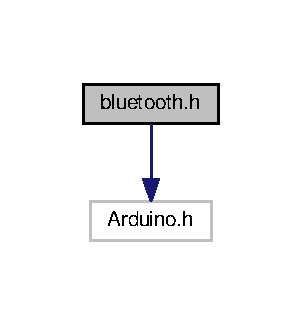
\includegraphics[width=145pt]{bluetooth_8h__incl}
\end{center}
\end{figure}
\subsection*{Třídy}
\begin{DoxyCompactItemize}
\item 
class \hyperlink{class_bluetooth}{Bluetooth}
\end{DoxyCompactItemize}


\subsection{Detailní popis}
Hloušek Matěj (\href{mailto:matej.hlousek@email.cz}{\tt matej.\+hlousek@email.\+cz}) \begin{DoxyDate}{Datum}
Listopad,2016
\end{DoxyDate}
\hyperlink{class_bluetooth}{Bluetooth} class. Třída přistupuje k bluetooth modulu 
\hypertarget{drivers_8h}{}\section{Dokumentace souboru drivers.\+h}
\label{drivers_8h}\index{drivers.\+h@{drivers.\+h}}
\subsection*{Definice maker}
\begin{DoxyCompactItemize}
\item 
\#define {\bfseries M\+A\+X\+\_\+\+E\+C\+H\+O\+\_\+\+T\+I\+ME}~5000\hypertarget{drivers_8h_a0850c94f39327239387d14f77eadfd26}{}\label{drivers_8h_a0850c94f39327239387d14f77eadfd26}

\item 
\#define {\bfseries M\+I\+N\+\_\+\+E\+C\+H\+O\+\_\+\+T\+I\+ME}~200\hypertarget{drivers_8h_a3f9c2525583900923a0ad646ff05a158}{}\label{drivers_8h_a3f9c2525583900923a0ad646ff05a158}

\item 
\#define {\bfseries N\+O\+\_\+\+E\+C\+HO}~0\hypertarget{drivers_8h_a30970a858be8016e6d5cc2dd68b5a324}{}\label{drivers_8h_a30970a858be8016e6d5cc2dd68b5a324}

\end{DoxyCompactItemize}
\subsection*{Funkce}
\begin{DoxyCompactItemize}
\item 
unsigned int \hyperlink{drivers_8h_a2178beb9a44da0d82e94345214ee9cf8}{read\+H\+C\+S\+R04} (int trigger\+Pin, int echo\+Pin)
\end{DoxyCompactItemize}


\subsection{Detailní popis}
Hloušek Matěj (\href{mailto:matej.hlousek@email.cz}{\tt matej.\+hlousek@email.\+cz}) \begin{DoxyDate}{Datum}
Listopad,2016
\end{DoxyDate}
drivers class. Třída pro přístup k modulům 

\subsection{Dokumentace funkcí}
\index{drivers.\+h@{drivers.\+h}!read\+H\+C\+S\+R04@{read\+H\+C\+S\+R04}}
\index{read\+H\+C\+S\+R04@{read\+H\+C\+S\+R04}!drivers.\+h@{drivers.\+h}}
\subsubsection[{\texorpdfstring{read\+H\+C\+S\+R04(int trigger\+Pin, int echo\+Pin)}{readHCSR04(int triggerPin, int echoPin)}}]{\setlength{\rightskip}{0pt plus 5cm}unsigned int read\+H\+C\+S\+R04 (
\begin{DoxyParamCaption}
\item[{int}]{trigger\+Pin, }
\item[{int}]{echo\+Pin}
\end{DoxyParamCaption}
)}\hypertarget{drivers_8h_a2178beb9a44da0d82e94345214ee9cf8}{}\label{drivers_8h_a2178beb9a44da0d82e94345214ee9cf8}
funkce k čtení vzdálenost z sonaru 
\begin{DoxyParams}{Parametry}
{\em trigger\+Pin} & \\
\hline
{\em echo\+Pin} & \\
\hline
\end{DoxyParams}
\begin{DoxyReturn}{Návratová hodnota}

\end{DoxyReturn}

\hypertarget{ibt_8h}{}\section{Dokumentace souboru ibt.\+h}
\label{ibt_8h}\index{ibt.\+h@{ibt.\+h}}
\subsection*{Třídy}
\begin{DoxyCompactItemize}
\item 
class \hyperlink{class_ibt}{Ibt}
\end{DoxyCompactItemize}


\subsection{Detailní popis}
Hloušek Matěj (\href{mailto:matej.hlousek@email.cz}{\tt matej.\+hlousek@email.\+cz}) \begin{DoxyDate}{Datum}
Listopad,2016
\end{DoxyDate}
I\+BT class. Třída přistupuje k regulátoru napětí pro motory 
\hypertarget{sekacka_8h}{}\section{Dokumentace souboru sekacka.\+h}
\label{sekacka_8h}\index{sekacka.\+h@{sekacka.\+h}}
\subsection*{Třídy}
\begin{DoxyCompactItemize}
\item 
class \hyperlink{class_sekacka}{Sekacka}
\end{DoxyCompactItemize}


\subsection{Detailní popis}
Hloušek Matěj (\href{mailto:matej.hlousek@email.cz}{\tt matej.\+hlousek@email.\+cz}) \begin{DoxyDate}{Datum}
Listopad,2016
\end{DoxyDate}
Seki class. Třída přistupuje k zařízením sekačky a stará se o ovlád 
%--- End generated contents ---

% Index
\backmatter
\newpage
\phantomsection
\clearemptydoublepage
\addcontentsline{toc}{chapter}{Rejstřík}
\printindex

\end{document}
